\begin{frame}
    \frametitle{Filtro de Partículas (Particle Filter)}
    \note{Información extraída de Vídeo de Cyrill Stachniss https://youtu.be/MsYlueVDLI0}
    \footnotesize
    \begin{itemize}
        \item Con EKF estamos restringidos a distribuciones Gaussianas.
        \item Cuando usamos EKF obtenemos una Distibuión Gaussiana que describe dónde se encuentra el robot.
        \item En Particle Filter utilizamos partículas o hipótesis que describen dónde podría estar el robot.
        \item En vez de tener una forma paramétrica como es EKF, que describimos la distribución de probabilidad con los parámetros media $\mu$ y covarianza $\covariance$. Partible Filter utiliza muestras no-paramétricas como hipótesis sobre dónde el robot podría estar.
    \end{itemize}
    
    
   	\begin{center}
        \movie[loop]{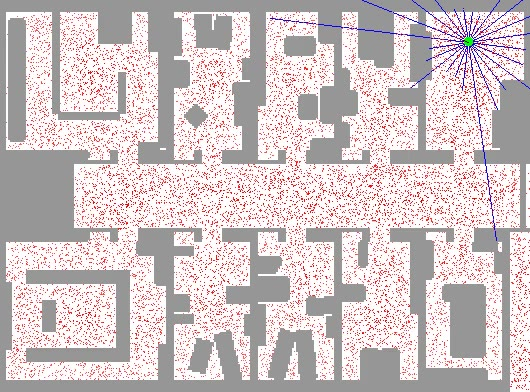
\includegraphics[width=0.4\columnwidth]{images/particle_filter/particle_filter_video.jpg}}{videos/particle_filter.mp4}
    \end{center}
    
    \note{Vídeo extraído de https://rse-lab.cs.washington.edu/projects/mcl/animations/global-floor.gif}
    
\end{frame}

\begin{frame}
    \frametitle{Aproximación flexible de una Función}
    \note{Información extraída de Vídeo de Cyrill Stachniss https://youtu.be/MsYlueVDLI0}
    \footnotesize
    
    \begin{itemize}
        \item Objetivo: Enfoque que nos permita estimar cualquier \textbf{distribución de probabilidad arbitraria}.
    \end{itemize}
    
    \begin{center}
    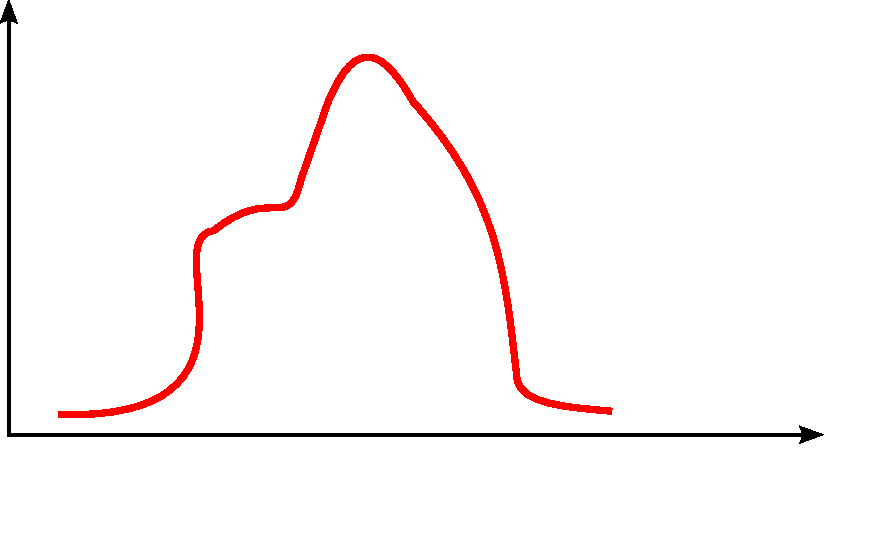
\includegraphics[width=0.5\columnwidth]{./images/particle_filter/arbitrary_distribution.pdf}
    \end{center}
    
\end{frame}

\begin{frame}
    \frametitle{Utilizando Muestras (Partículas)}
    \note{Información extraída de Vídeo de Cyrill Stachniss https://youtu.be/MsYlueVDLI0}
    \footnotesize
    \begin{itemize}
        \item \textbf{Múltiples muestras} para representar una distribución de probabilidad arbitraría
        \item Las muestras están más agrupadas en algunas áreas y en otras menos. La cantidad de partículas por unidad de área describe que tan probable es que el robot se encuentre en esa área.
        \item Cada muestra está acumulando un poco de ``masa de probabilidad''.
        \item Las muestra puede ser vista como una aproximación a la función de densidad de probabilidad (pdf).
        \item Para obtener la pdf, hay que integrar sobre una cierta área de manera de obtener la masa de probabilidad de que el robot se encuentre en dicha área. 
        \item Por tanto, en los lugares donde la pdf sea alta tendremos más partículas, y en los lugares donde la pdf tenga valores bajos tendremos menos partículas.
    \end{itemize}
    
    \begin{center}
    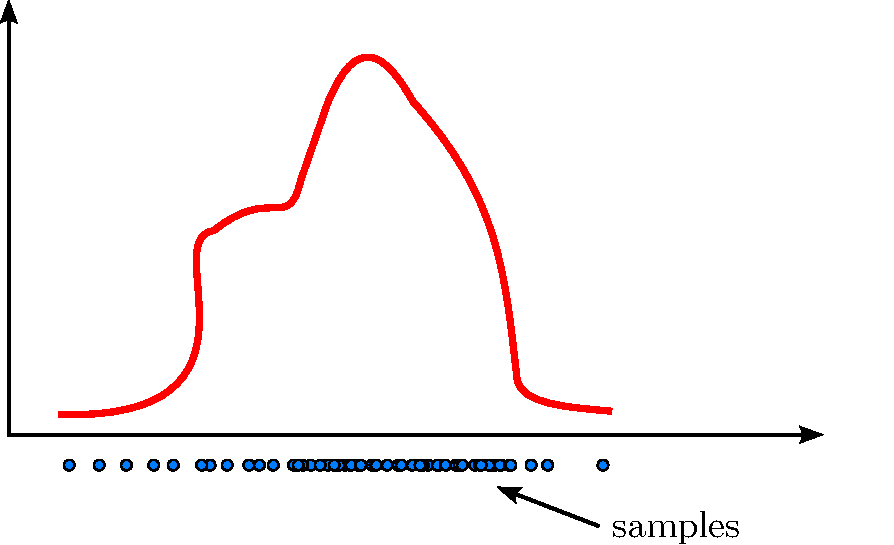
\includegraphics[width=0.5\columnwidth]{./images/particle_filter/arbitrary_distribution_samples.pdf}
    \end{center}
    
\end{frame}

\begin{frame}
    \frametitle{Utilizando Muestras con Peso}
    \note{Información extraída de Vídeo de Cyrill Stachniss https://youtu.be/MsYlueVDLI0}
    \footnotesize
    \begin{itemize}
        \item En vez de utlizar la acumulación de muestras para representar una distribución de probabilidad arbitraría, podemos utilizar \textbf{Múltiples muestras con peso} 
        \item Es posible reducir el número de muestras que necesitamos, si le agregamos pesos a cada muestra
        \item Mientras más peso tiene una muestra, más masa de probabilidad hay en esa región
        \item Los pesos de todas las muestras juntas deben sumar 1
        \item Al inicio, podríamos agregarle a cada muestra un peso uniforme. Por ejemplo, si tenemos $n$ muestras, entonces cada muestra tiene peso $\frac{1}{n}$
    \end{itemize}
    
    \begin{center}
        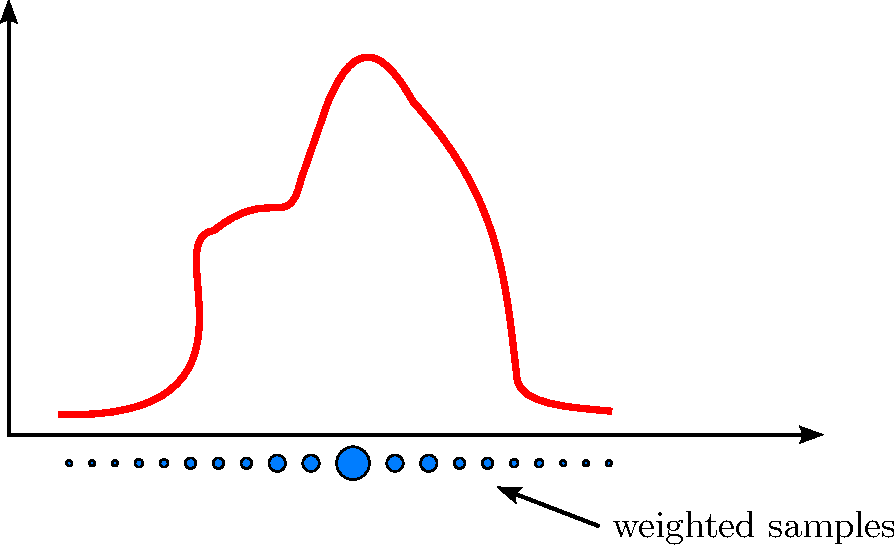
\includegraphics[width=0.5\columnwidth]{./images/particle_filter/arbitrary_distribution_weighted_samples.pdf}
    \end{center}
    
\end{frame}

\begin{frame}
    \frametitle{Filtro de Partículas (Particle Filter)}
    \note{Información extraída de Vídeo de Cyrill Stachniss https://youtu.be/MsYlueVDLI0}
    
    \footnotesize
    \begin{itemize}
        \item Notar que es una aproximación de la PDF (\emph{Probabilistic Density Function})
        \item Es importante tener un número de muestras suficientes para poder representar la PDF adecuadamente.
    \end{itemize}
    
    
\end{frame}

\begin{frame}
    \frametitle{Conjunto de Partículas}
    \note{Información extraída de Vídeo de Cyrill Stachniss https://youtu.be/MsYlueVDLI0}
    
    \begin{itemize}
        \item Conjunto de partículas con peso
            
        \begin{center}
            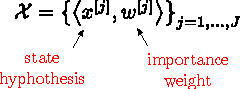
\includegraphics[width=0.5\columnwidth]{./images/particle_filter/weighted_samples.pdf}
        \end{center}

        \item Las partículas representan la posterior belief dada por
        \begin{equation*}
            p(x) = \sum_{j=1}^{J} w^{[j]} \delta_{x^{[j]}}(x)    
        \end{equation*}
        donde $\delta_{x^{[j]}}(x)$ es la función de Dirac centrada en la ubicación de la partícula $x^{[j]}$.

        \begin{equation*}
            \delta(y) = 
            \begin{cases} 
            \infty, & y = x^{[j]} \\ 
            0, & y \neq x^{[j]} 
            \end{cases};    
        \end{equation*}

        \note{La función de Dirac simula impulsos o eventos}
        \note{La función de Dirac tiende a infinito cuando $x=j$ y, para cualquier otro valor de $x$, es igual a 0.}

        \note{Vamos a necesitar un mayor número de partículas mientras más compleja es la fdp}

    \end{itemize}
   
\end{frame}


\begin{frame}
    \frametitle{Partículas para Aproximar}
    \note{Información extraída de Vídeo de Cyrill Stachniss https://youtu.be/MsYlueVDLI0}
    
    \begin{itemize}
        \item Partículas para aproximar una función
        
        \begin{center}
            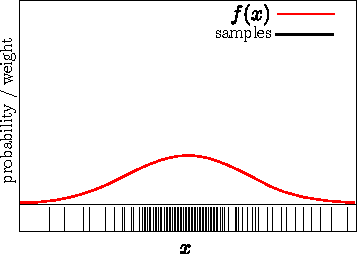
\includegraphics[width=0.45\columnwidth]{./images/particle_filter/gaussian_approximation_by_sampling.pdf}
            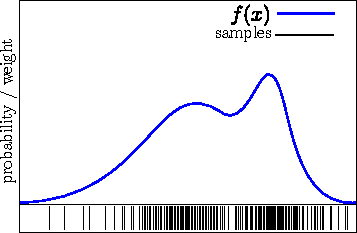
\includegraphics[width=0.45\columnwidth]{./images/particle_filter/particles_for_approximation.pdf}
        \end{center}

        \item Más partículas caen en una región, más alta es la probabilidad de la región
    \end{itemize}
    
    \begin{center}
        \alert{¿Cómo obtener dichas muestras?}
    \end{center}

    \note{Cómo obtener las muestras es un problema. En general no podemos obtener muestra de forma cerrada de una función arbitraria. Hay pocas funciones de las que podemos hacer sampleo de forma cerrada o mostrar de manera eficiente. Por ejemplo, si tenemos que aproximar una distribución uniforme donde todo los estados tienen la misma probabilidad entonces podemos utilizar una función de generación de números aleatorios como es el caso de la función rand() en C.}
    \note{Para el caso de una distribución gaussiana, generar número de manera aleatoria no nos sirve. Tenemos que poder generar más números serca de la media.}

\end{frame}

\begin{frame}
    \frametitle{Una Forma Cerrada de Muestreo es solo posible para Pocas Distribuciones}
    \note{Información extraída de Vídeo de Cyrill Stachniss https://youtu.be/MsYlueVDLI0}

    \begin{itemize}
        \item Ejemplo: Muestreo de una Distribución Gaussiana
    \end{itemize}

    \begin{figure}
        \begin{minipage}[m]{.5\textwidth}
            \raggedright
            \begin{center}
                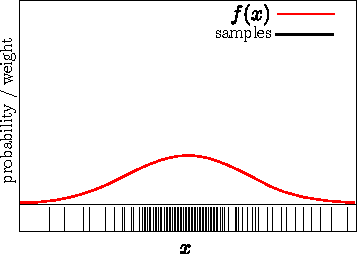
\includegraphics[width=\columnwidth]{./images/particle_filter/gaussian_approximation_by_sampling.pdf}
            \end{center}
        \end{minipage}% <---------------- Note the use of "%"
        \begin{minipage}[m]{.5\textwidth}
            \raggedleft
            \centering
            \begin{equation*}
                x \leftarrow \frac{1}{2} \sum_{i=1}^{12} \text{rand}(-\sigma, \sigma)    
            \end{equation*}

            \note{Al dividir por 2 estamos generando muestras desde -6 simga a 6 sigma lo cúal aproxima bastante bien la distribución gaussiana pero no es exacta.}
        \end{minipage}
    \end{figure}

    ¿Cómo samplear utilizando otra distribución?

    \note{Técnica de rejection sampling. No sé utiliza en particle filter porque es una técnica muy ineficiente.}

    \note{Técnica Importance Sampling Principle}

\end{frame}
    


\begin{frame}
    \frametitle{Importance Sampling Principle}
    \note{Información extraída de Vídeo de Cyrill Stachniss https://youtu.be/MsYlueVDLI0}

    \scriptsize

    \begin{itemize}
        \item Podemos usar una distribución diferente $\pi$ para generar muestras de una distribución $f$ (la cuál queremos utilizar realmente para hacer el muestreo)
        \item Considere las ``diferencias entre $\pi$ y $f$'' usando un peso $w = f(x) / \pi(x)$
        \item Función de Distribución objetivo (\emph{target}) $f$
        \item Función de Distribución propuesta (\emph{Proposal}) $\pi$
        \item Precondición:
        $f(x) > 0 \implies \pi(x) > 0$
        \note{La precondición es requerida dado que si hay un caso donde f(x) > 0 y pi(x) < 0, significa que hay probabilidad cero de generar esa muestra con la función pi (proposal) y por tanto nunca podremos generar una muestra para f (target). No pudiendo aproximar adecuadamente f. Además, se puede ver que para el calculo de los pesos w, si pi(x) = 0 entonces tendríamos un peso indefinido (infinito), que no es algo que queremos.}
        \begin{center}
        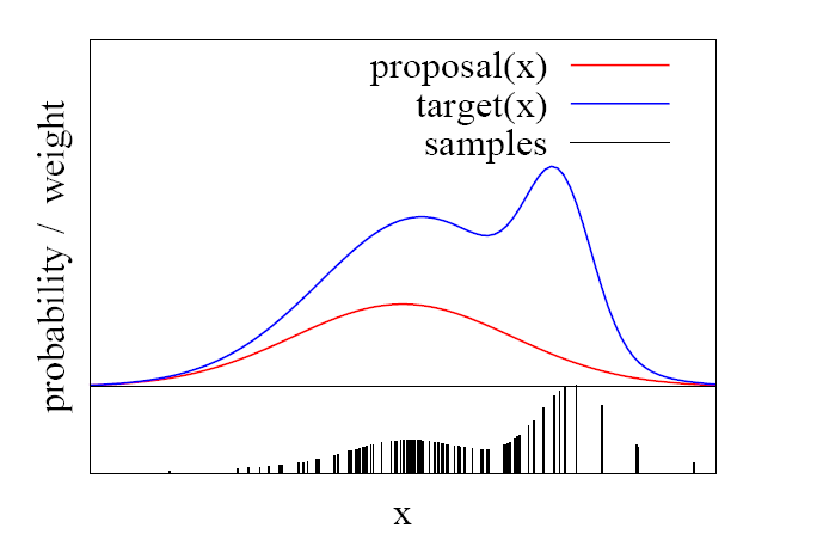
\includegraphics[width=0.4\textwidth]{./images/particle_filter/importance_sampling_principle.pdf}
        \end{center}
        Mientras más diferencia hay entre el valor de la función $target$ y la función $proposal$, más peso se le asigna a la muestra (rayas más altas). Observar que la función proposal determina la frecuencia de las muestras. En este caso, para la parte más alta de la función target, hay pocas muestras pero estas tienen un peso alto.

    \end{itemize}

    \note{El Importance Sampling Principle nos dice que podemos usar una distribución proposal para generar muestras de una distribución target (para la cuál queremos realmente hacer el muestreo) compensando las equivocaciones que cometamos. Y las equivocaciones aquí significa la diferencia entre los valores de la curva roja y la curva azul. Para esto debemos poder evaluar la función proposal y la función target para la misma entrada, y calcular el peso w. Los pesos sirven para compenzar.}

\end{frame}
    
\begin{frame}
    \frametitle{Filtro de Partículas para problemas de estimación de estado dinámico}
    \note{Información extraída del Vídeo de Cyrill Stachniss https://youtu.be/MsYlueVDLI0}

    \begin{itemize}
        \item PF implementa un Filtro Bayesiano Recursivo (realiza un Prediction step y un Correction step)
        \item Enfoque no paramétrico (permite trabajar con distribuciones no gaussianas)
        \item Modela la distribución mediante muestras
        \item \textbf{Predicción}: extraer de la distribución \emph{proposal}
        \item \textbf{Corrección}: ponderación con el ratio entre la distribución \emph{target} y la \emph{proposal}
        \item \alert{¡Cuantas más muestras usemos, mejor será la estimación!}
    \end{itemize}
\end{frame}
    
\begin{frame}
    \frametitle{Algoritmo de Filtro de Partículas}
    \note{Información extraída de Vídeo de Cyrill Stachniss https://youtu.be/MsYlueVDLI0}

    \begin{enumerate}
        \item Muestrear las partículas utilizando la distribución \emph{proposal}.
        \begin{equation*}
            x_{t}^{[j]} \sim proposal(x_{t} | \ldots) \qquad \text{(análogo a tomar muestras de la curva roja)}
        \end{equation*}
        \item Calcular los pesos de importancia
        \begin{equation*}
            w_t^{[j]} = \frac{target(x_t^{[j]})}{proposal(x_t^{[j]})} \qquad \text{{(pesos para compesar las diferencias entre \emph{proposal} y \emph{target})}}
        \end{equation*}
        \item Resampling: Tomar la partícula $i$ con probabilidad $w_{t}^{[j]}$ y repetir $J$ veces.
        \note{observar que en el resampling estamos reemplazando el peso de una muestra por la frecuencia de esta muesta. Es decir, mientras mas peso tenga una muestra mas veces la elegiremos.}

        \note{También, en el reesampling al elegir muestras con mayor peso y al no elegir muestras con poco peso estamos describiendo mejor la probability distribution mass ya que las partículas de poco peso no contribuyen mucho a la probability distribution mass, y permite hacer un uso mejor de la memoria de la computadora.}
        
        (es decir, generamos muestras compensando)
    \end{enumerate}
    \note{Reemplazar muestras improbables por otras más probables}

    \vspace{1cm}

    Intepretando PF con el Filtro de Bayes Recursivo:
    \begin{itemize}
        \item Paso 1 se corresponde con el Paso de Predicción utilizando el modelo de movimiento y,
        \item Pasos 2 y 3 se corresponden con el Paso de Corrección utilizando el modelo de observación para el cálculo de los pesos.
    \end{itemize}

\end{frame}

\begin{frame}
    \frametitle{Algoritmo de Filtro de Partículas}
    \note{Información extraída de Vídeo de Cyrill Stachniss https://youtu.be/MsYlueVDLI0}

    \begin{algorithmic}[1]
    \Procedure{ParticleFilter}{$\mathcal{X}_{t-1}, u_{t}, z_{t}$}:
    \State $\bar{\mathcal{X}}_t = \mathcal{X}_t = \emptyset$
    \For{$j = 1$ to $J$}
        \State sample $x_t^{[j]} \sim \pi(x_t)$
        \State $w_t^{[j]} = \dfrac{p(x_t^{[j]})}{\pi(x_{t}^{[j]})}$
        \State $\bar{\mathcal{X}}_t = \bar{\mathcal{X}}_t + \langle x_t^{[j]}, w_t^{[j]}\rangle$
    \EndFor
    \For{$j = 1$ to $M$}
        \State Draw $i$ with probability $\propto w_t^{[i]}$
        \State Add $x_t^{[i]}$ to $\mathcal{X}_t$
    \EndFor
    \State return $\mathcal{X}_t$
    \EndProcedure
    \end{algorithmic}
\end{frame}


\begin{frame}
    \frametitle{Monte Carlo Localization}
    \note{Información extraída de Vídeo de Cyrill Stachniss https://youtu.be/MsYlueVDLI0}

    Monte Carlo Localization: Filtro de Partículas para la localización de un robot.

\end{frame}


% \begin{frame}
%     \frametitle{Monte Carlo Localization}

%     \begin{center}
%         \includegraphics[width=0.37\textwidth]{./images/particle_filter/monte_carlo_localization_example.pdf}
%     \end{center}

% \end{frame}

\begin{frame}
    \frametitle{Monte Carlo Localization}
    \note{Información extraída de Vídeo de Cyrill Stachniss https://youtu.be/MsYlueVDLI0}

    \begin{itemize}
        \item Cada partícula es una hipótesis de la pose
        \item \emph{Proposal} es el motion model
        \begin{equation*}
            \state_t^{[j]} \sim p(\state_{t} \, | \, \state_{t-1}, \controlCommand_{t})
        \end{equation*}

        Aquí, muestreamos desde la distribución \emph{proposal} $p(\state_{t} \, | \, \state_{t-1}, \controlCommand_{t})$. Notar que como $\controlCommand_{t}$ tiene ruido cada partícula se mueve con cierta diferencia. Por ejemplo, si $\controlCommand_{t}$ dice que el robot se movió \SI{1}{\meter} entonces habrá una partícula que se mueva \SI{0.97}{\meter}, otra \SI{1.02}{\meter}, etc.

        \item Corrección vía el observation model 
        \begin{equation*}
            w_t^{[j]} = \frac{target}{proposal} \propto p(z_t \, | \, x_t, m)
        \end{equation*}
        \note{es proporcional porque normalizamos los pesos a que sus suma sea 1.}
    \end{itemize}
\end{frame}

    
\begin{frame}
    \frametitle{Filtro de Partículas para Localización}
    \note{Información extraída de Vídeo de Cyrill Stachniss https://youtu.be/MsYlueVDLI0}

    \begin{algorithmic}[1]
        \Procedure{ParticleFilter}{$\mathcal{X}_{t-1}, u_{t}, z_{t}$}
        \State $\bar{\mathcal{X}}_t = \mathcal{X}_t = \emptyset$
        \For{$j = 1$ to $J$}
            \State Sample \alert{$x_t^{[j]} \sim p(x_t \, | \, u_t, x_{t-1}^{[j]})$}
            \State $w_t^{[j]} = \alert{p(z_t \, | \, x_t^{[j]})}$
            \State $\bar{\mathcal{X}}_t = \bar{\mathcal{X}}_t + \langle x_t^{[j]}, w_t^{[j]}\rangle$
        \EndFor
        \For{$i = 1$ to $J$}
            \State Draw $i \in 1,\ldots,J$ with probability $\propto w_t^{[i]}$
            \State Add $x_t^{[i]}$ to $\mathcal{X}_t$
        \EndFor
        \State return $\mathcal{X}_t$
    \EndProcedure
    \end{algorithmic}
\end{frame}
    
\begin{frame}
    \frametitle{Monte Carlo Localization - Paso de Corrección}
    \note{Información extraída de Vídeo de Cyrill Stachniss https://youtu.be/MsYlueVDLI0}

    \begin{center}
        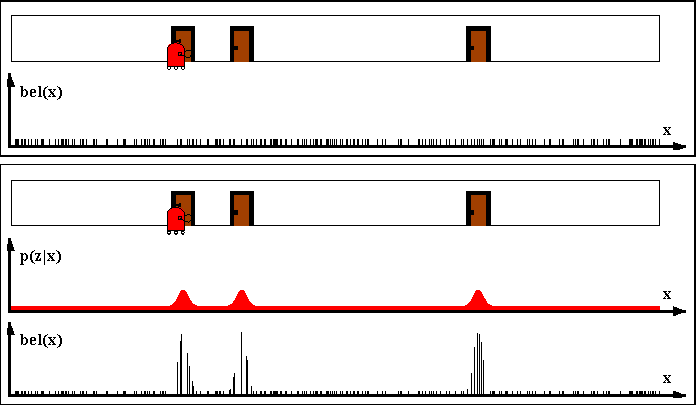
\includegraphics[width=0.8\textwidth]{./images/particle_filter/monte_carlo_correction.pdf}
    \end{center}

\end{frame}

\begin{frame}
    \frametitle{Monte Carlo Localization - Remuestreo y Predicción}
    \note{Información extraída de Vídeo de Cyrill Stachniss https://youtu.be/MsYlueVDLI0}

    \begin{center}
        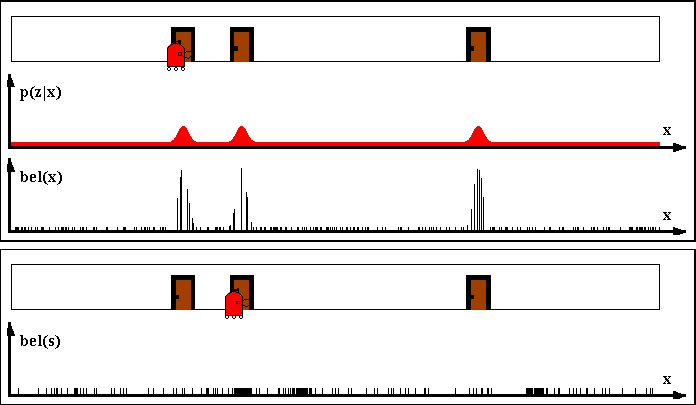
\includegraphics[width=0.8\textwidth]{./images/particle_filter/monte_carlo_resample_and_predict.pdf}
    \end{center}

\end{frame}

\begin{frame}
    \frametitle{Monte Carlo Localization - Paso de Corrección 2}
    \note{Información extraída de Vídeo de Cyrill Stachniss https://youtu.be/MsYlueVDLI0}

    \begin{center}
        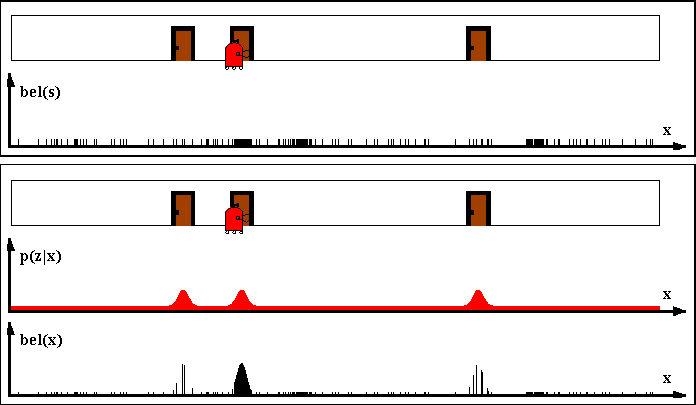
\includegraphics[width=0.8\textwidth]{./images/particle_filter/monte_carlo_correction2.pdf}
    \end{center}

\end{frame}

\begin{frame}
    \frametitle{Monte Carlo Localization - Remuestreo y Predicción 2}
    \note{Información extraída de Vídeo de Cyrill Stachniss https://youtu.be/MsYlueVDLI0}

    \begin{center}
        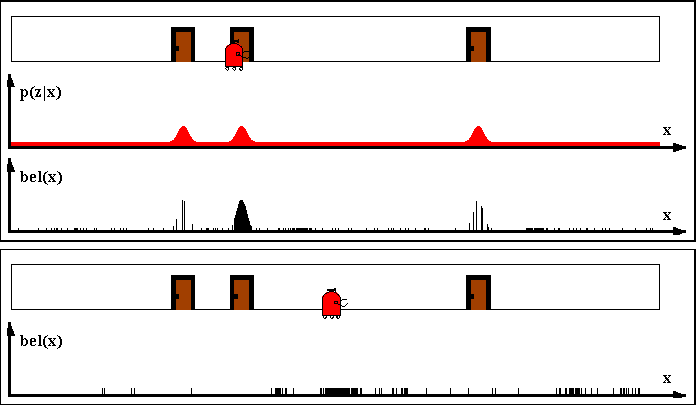
\includegraphics[width=0.8\textwidth]{./images/particle_filter/monte_carlo_resample_and_predict2.pdf}
    \end{center}

\end{frame}


\begin{frame}
    \frametitle{Resampling}
    \note{Información extraída de Vídeo de Cyrill Stachniss https://youtu.be/MsYlueVDLI0}

    \note{El Resampling se encarga de reemplazar partículas poco probables por partículas más probables porque no queremos gastar memoria en áreas que no importan. Para esto toma partículas proporcionalmente a su peso haciendo que las partículas con mucho peso sean elegidas muchas veces y las de poco peso no.}

    \begin{itemize}
        \item Tomar la partícula $i$ con probabilidad $w_t^{[i]}$. Repetir $J$ veces.
        \item Informalmente: ``Reemplazar muestras improbables por otras más probables''
        \item Supervivencia del más apto
        \item ``Truco'' para evitar que muchas muestras cubran estados improbables
        \item Necesario, ya que tenemos un número limitado de muestras (memoria finita)
    \end{itemize}
\end{frame}
    
\begin{frame}
    \frametitle{Métodos de Resampling}
    \note{Información extraída de Vídeo de Cyrill Stachniss https://youtu.be/MsYlueVDLI0}

    \scriptsize

    
    \only<1>{
        \begin{center}
            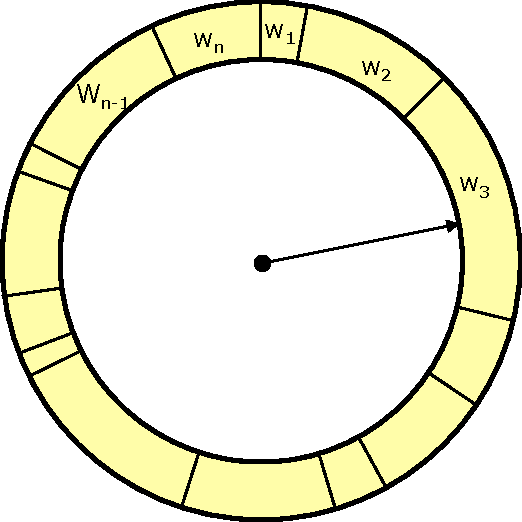
\includegraphics[width=0.3\textwidth]{./images/particle_filter/resampling_rulette_wheel1.pdf}
        \end{center}
    }
    \only<2>{
        \begin{center}
            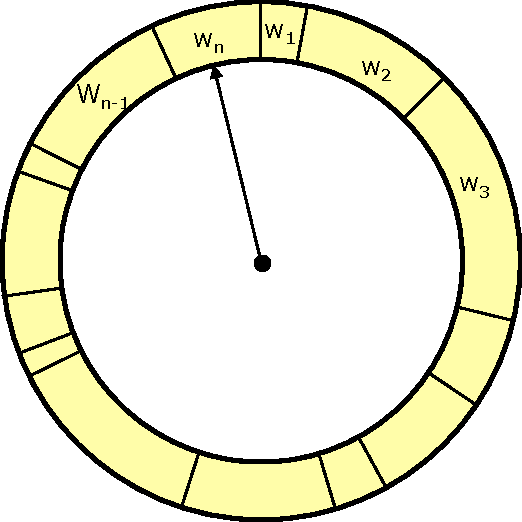
\includegraphics[width=0.3\textwidth]{./images/particle_filter/resampling_rulette_wheel2.pdf}
        \end{center}
    }
    \only<3>{
        \begin{center}
            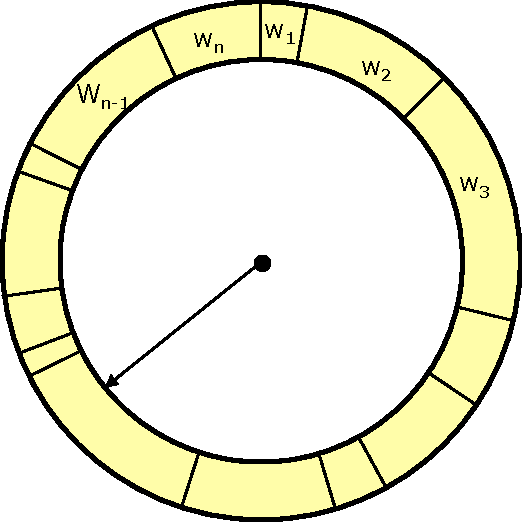
\includegraphics[width=0.3\textwidth]{./images/particle_filter/resampling_rulette_wheel3.pdf}
        \end{center}
    }
    \begin{itemize}
        \item Roulette Wheel
        \item Los buckets de la ruleta representan los pesos de las partículas. Mientras más grande el bucket, más probable es que esta partícula sea seleccionada.
        \item Tenemos que hacerlo $J$ veces. Tenemos que encontrar dónde cae la bola. Esto lo podemos hacer con Búsqueda binaria. La suma de todos los pesos de la ruleta es 1. Si tiramos un número random entre 0 y 1 entonces con búsqueda binaria podemos saber en qué bucket cae.
        \item Búsqueda binaria para saber en qué bucket cae la bola ($O(J \log(J))$)
    \end{itemize}

\end{frame}

\begin{frame}
    \frametitle{Métodos de Resampling}
    \note{Información extraída de Vídeo de Cyrill Stachniss https://youtu.be/MsYlueVDLI0}

    \footnotesize

    \only<1>{
        \begin{center}
            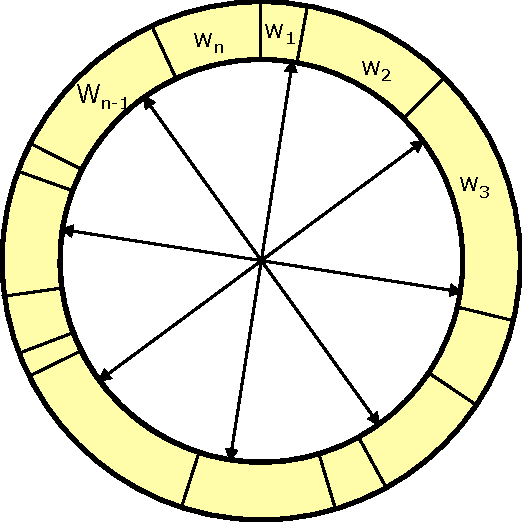
\includegraphics[width=0.3\textwidth]{./images/particle_filter/resampling_stochastic_universal_sampling1.pdf}
        \end{center}
    }
    \only<2>{
        \begin{center}
            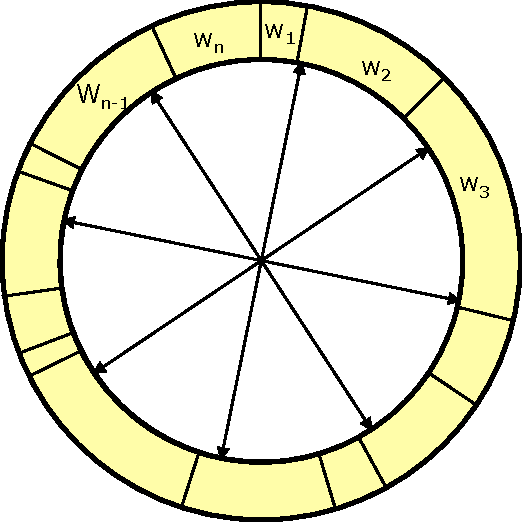
\includegraphics[width=0.3\textwidth]{./images/particle_filter/resampling_stochastic_universal_sampling2.pdf}
        \end{center}
    }

    \begin{itemize}
        \item Stochastic universal sampling (utilizando $J$ flechas equidistantes)
        \item También llamado \emph{Low-Variance Resampling} (evita que las partículas se concentren rápidamente)
        \item Utilizando J flechas y poniendolas equidistantes. Rotamos todas juntas y elejimos de a J partículas. Por tanto cuando, tiro un número random ahora se seleccionan las J partículas de una.
        \item Tiene costo computacional lineal $O(J)$ porque solo tengo que recorrer los pesos una vez para ver dónde caen todas las flechas.
    \end{itemize}

    \note{Ejemplo 8 flechas distante 45 grados una de otra.}
\end{frame}

\begin{frame}
    \frametitle{Resampling}
    \note{Información extraída de Vídeo de Cyrill Stachniss https://youtu.be/MsYlueVDLI0}

    \begin{itemize}
        \item Muestreo con remplazo (muestreamos tomando una partícula y luego la volvemos a colocar en la bolsa)
        \item Roulette Wheel resampling es fácil de entender pero es subóptimo en la práctica
        \item \alert{¿Qué pasa si todas las partículas tienen el mismo peso?}
        \note{Si todas las partículas tienen el mismo peso, sería como tener un sensor que no me da información.}
        \note{Si todas las partículas tienen el mismo peso, el resampling seleccionará partículas de manera aleatoria y las duplicará, y otras partículas no serán seleccionadas y moriran. Y esto pasa sin que una partícula sea mejor que otra. Esto lleva a que el sistema converja en una localización cualquiera.}
        \note{Por tanto, si todas las partículas tienen el mismo peso entonces no tiene sentido escoger una por encima de otra.}

        \note{
            https://robotics.stackexchange.com/questions/16093/why-does-the-low-variance-resampling-algorithm-for-particle-filters-work

            TLDR; A particle filter’s convergence rate is inversely proportional to the variance in the parents’ offspring counts. Low variance means fast convergence.

            NOTE: Below, I discuss (but never explicitly mention) the concept of variance effective population size.

            The effectiveness of this resampling strategy makes a lot of sense when you consider that the particle filter is, at its core, an evolutionary algorithm (EA). All EAs tend to lose diversity because of the random sampling step, at a rate proportional to the variance in how many offspring the parents produce. This effect is known as genetic drift, and it adversely affects biological populations as well. As a result of this diversity loss, the EA prematurely converges to suboptimal solutions. This is bad news.

            Intuitively, genetic drift makes sense. When parents are chosen at random (the most common setup), those with low fitness/quality are likely to get skipped and produce zero offspring and be eliminated from the gene pool, thus reducing the population’s diversity. Now, the rate at which natural selection improves a population’s fitness is directly proportional to the population’s diversity—diversity is literally the fuel that drives natural selection. Genetic drift reduces the the diversity, thus decreasing the rate at which the population’s fitness can improve and causing the aforementioned bad news.

            Let’s now look at the low-variance resampling method. This method gives almost every parent exactly the number of offspring that they would be expected to get with the random sampling, without the extra uncertainty (variance). This reduces genetic drift and greatly increases the efficiency with which the particle filter can improve its solution and/or adapt to changing condition
        }

    \end{itemize}
\end{frame}


\begin{frame}
    \frametitle{Idea de Low Variance Resampling}
    \note{Información extraída de Vídeo de Cyrill Stachniss https://youtu.be/MsYlueVDLI0}

    \begin{center}
        \only<1>{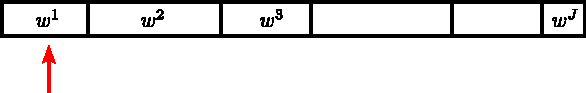
\includegraphics[width=0.7\textwidth]{./images/particle_filter/low_variance_resampling1.pdf}}
        \only<2>{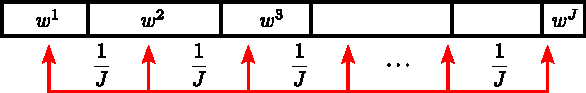
\includegraphics[width=0.7\textwidth]{./images/particle_filter/low_variance_resampling2.pdf}}
    \end{center}

    \begin{enumerate}
        \item<1-> Tomamos un valor random $r$ entre 0 y $\dfrac{1}{j}$
        \item<2> Tomamos $J-1$  partículas en $\dfrac{1}{J}$ pasos (basado en el peso acumulado)
    \end{enumerate}

\end{frame}

\begin{frame}
    \frametitle{Low Variance Resampling: Implementación eficiente}
    \note{Información extraída de Vídeo de Cyrill Stachniss https://youtu.be/MsYlueVDLI0}

    \begin{center}
        \only<1>{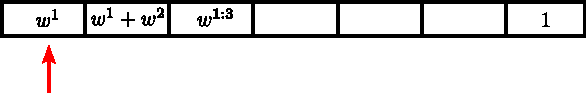
\includegraphics[width=0.7\textwidth]{./images/particle_filter/low_variance_resampling_efficient_implementation1.pdf}}
        \only<2>{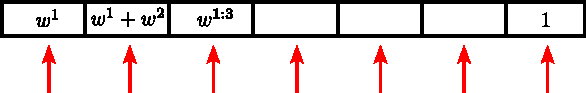
\includegraphics[width=0.7\textwidth]{./images/particle_filter/low_variance_resampling_efficient_implementation2.pdf}}
    \end{center}

    \begin{enumerate}
        \item<1-> Tomamos un valor random $r$ entre 0 y $\dfrac{1}{j}$
        \item<2>
        \begin{algorithmic}[1]
            \For{$j = 1$ to $J$}
                \State $U = r + (j - 1)  \dfrac{1}{J}$
                \While{$\left(U > cum[i]\right)$}
                    \State $i++$
                \EndWhile
                \State Add $x_t^{[i]}$ to $\bar{\mathcal{X}}_t$
            \EndFor
        \end{algorithmic}
        % \begin{fleqn}[\parindent]
        %     \begin{align*}
        %         for &(j=1 \dots J)\\
        %             &U = r + j \dfrac{1}{J}\\
        %             &while (U > cum[i]) \quad i++;\\
        %             &pick\_particle(i)
        %     \end{align*}
        % \end{fleqn}
    \end{enumerate}
    
\end{frame}

\begin{frame}
    \frametitle{Low Variance Resampling}

    \begin{algorithmic}[1]
        \Procedure{Low Variance Resampling}{$\mathcal{X}_{t}$,$\mathcal{W}_{t}$}
        \State $\bar{\mathcal{X}}_t = \emptyset$
        \State $r = \text{rand}(0; J^{-1})$
        \State $c = w_t^{[1]}$
        \State $i = 1$
        \For{$j = 1$ to $J$}
            \State $U = r + (j - 1)  J^{-1}$
            \While{$U > c$}
                \State $i = i + 1$
                \State $c = c + w_t^{[i]}$
            \EndWhile
            \State Add $x_t^{[i]}$ to $\bar{\mathcal{X}}_t$
        \EndFor
        \State Return $\bar{\mathcal{X}}_t$
        \EndProcedure
    \end{algorithmic}

    % \begin{tikzpicture}[remember picture,overlay]
    %     \node[xshift=-5.5cm,yshift=0.5cm] at (current page.east) { 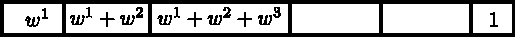
\includegraphics[width=0.6\textwidth]{./images/particle_filter/low_variance_resampling.pdf}};
    % \end{tikzpicture}

\end{frame}

\begin{frame}
    \frametitle{Low Variance Resampling}
    \note{Información extraída de Vídeo de Cyrill Stachniss https://youtu.be/MsYlueVDLI0}

    \begin{itemize}
        \item Realiza un remuestreo que mantiene las muestras en el caso que tengan pesos iguales
        \item Es más rápido que el remuestreo con roulette wheel: $O(J)$ vs. $O(J \log J)$
        \item \alert{Utilizaremos siempre Low Variance Resampling!}
    \end{itemize}
\end{frame}


\begin{frame}
    \frametitle{Desventajas de Particle Filter}
    \note{Información extraída de Vídeo de Cyrill Stachniss https://youtu.be/MsYlueVDLI0}

    \begin{itemize}
        \item No escala bien para espacios de alta dimensionalidad
        \note{PF se hace muy caro computacionalmente ya que necesitaremos muchas partículas para cubrir la distribución de probabilidad. PF funciona bien para bajas dimensiones, hasta 4 se puede pero más ya requiere tomar ciertas heurísticas para reducir el número de partículas y que estas sean representativas.}
        \note{El número de partículas crece exponencialmente con las dimenciones del estado}
        \item Problemático en situaciones con mucha incertidumbre
        \item \emph{Depletion Problem} (la mayoría de las partículas tienen poco peso)
        \note{El Depletion Problem: sucede cuando tenemos muy pocas partículas en comparación a la dimensionalidad del estado, las partículas no cubren las áreas de mayor probabilidad y por tanto mueren, haciendo que el filtro diverja eventualmente.
        Ejemplo: Imagina que tienes 100 partículas rastreando la posición de un robot. Si el robot da un giro brusco, muchas partículas tendrán pesos bajos porque no predicen bien el movimiento. Tras el resampling, solo unas pocas partículas "sobrevivirán", y el filtro perderá diversidad, afectando la estimación futura.}
    \end{itemize}
\end{frame}

\begin{frame}
    \frametitle{Ventajas}
    \note{Información extraída de Vídeo de Cyrill Stachniss https://youtu.be/MsYlueVDLI0}

    \begin{itemize}
        \item Puede trabajar con distribuciones no Gaussianas
        \item Funciona bien en espacios de baja dimensionalidad
        \item Puede manejar ambiguedades en la asociación de los datos \note{Podemos hacer que cada partícula tenga su propia forma de asociar datos. Como no hay incertidumbre asociada a esto, podemos hacer decisiones dependientes a cada partícula y ver qué partícula sobrevive.}
        \item Puede incorporar fácilmente diferentes modalidades de sensado \note{Podemos incorporar diferentes modalidades de sensado tan solo multiplicando el peso con el peso computado de otro sensor}
        \item Robusto \note{Robusto porque incluso cuando los modelos no sean perfectos será capaz de computar buenas belief}
        \item Fácil de implementar
    \end{itemize}
\end{frame}

\begin{frame}
    \frametitle{Resumen – Particle Filter}
    \note{Información extraída de Vídeo de Cyrill Stachniss https://youtu.be/MsYlueVDLI0}

    \begin{itemize}
        \item Los filtros de partículas son filtros bayesianos recursivos y no paramétricos
        \item El Posterior Belief se representa mediante un conjunto de muestras ponderadas
        \item No se limita a Distribuciones Gaussianas
        \item Proposal para extraer muestras en $t+1$
        \item Peso para tener en cuenta las diferencias entre la proposal y el target
        \item El arte está en diseñar modelos de movimiento y sensado adecuados
    \end{itemize}
\end{frame}
    
\begin{frame}
    \frametitle{Resumen – Localización con PF}
    \note{Información extraída de Vídeo de Cyrill Stachniss https://youtu.be/MsYlueVDLI0}

    \begin{itemize}
        \item Las partículas se propagan según el modelo de movimiento
        \item Se ponderan según la probabilidad de la observación
        \item Se denomina Localización de Monte Carlo (MCL)
        \item La MCL es un gold standard para la localización de robots móviles en entornos \emph{indoor}
    \end{itemize}
\end{frame}